\begin{figure}[ht]
	\centering
	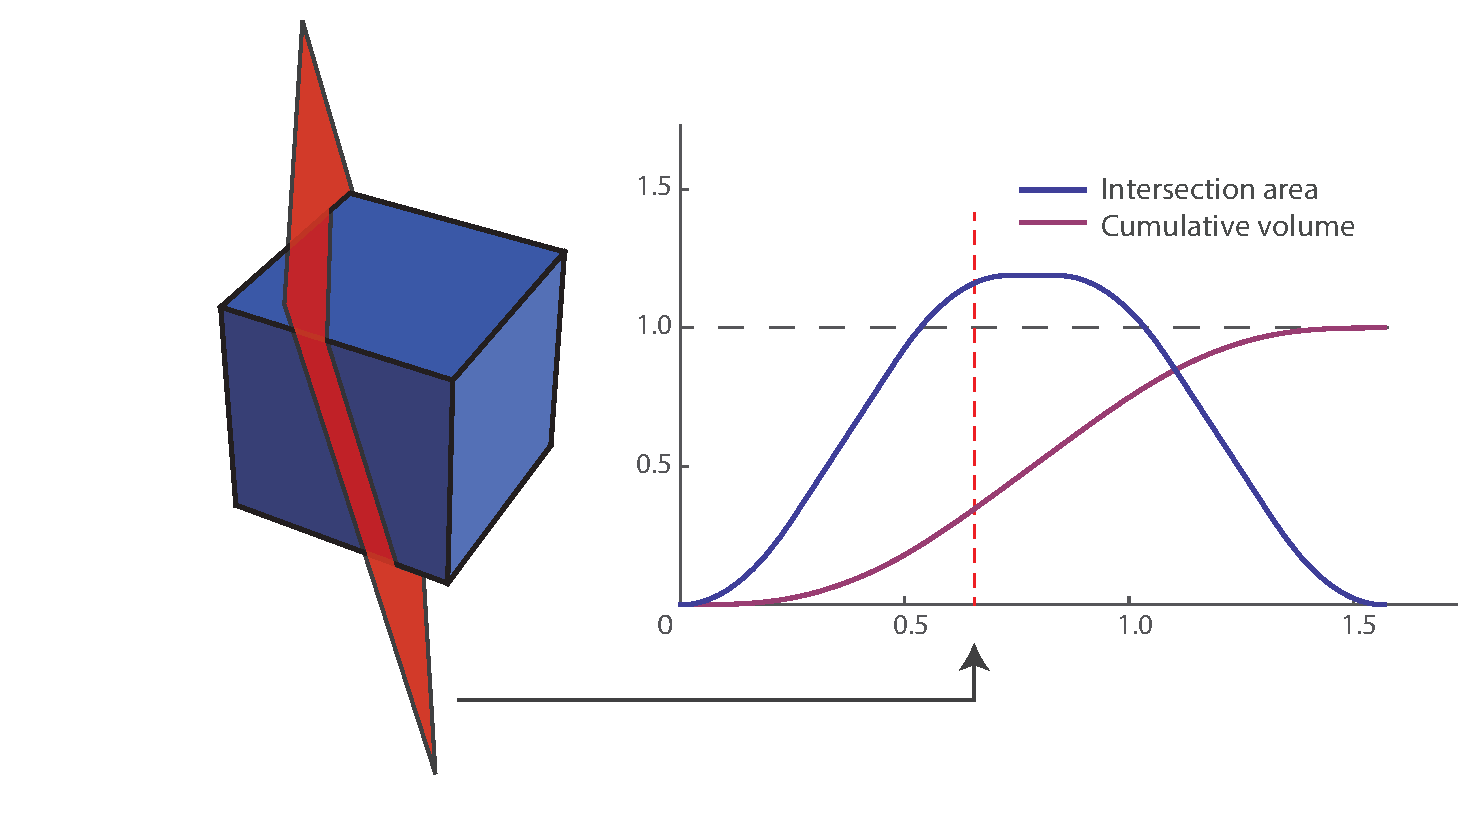
\includegraphics[width=1.\textwidth, clip=true]{./Chapters/03_GLM/./Images/Cube}
	\caption{The plane of arbitrary normal $\vec{n}$ (here $\vec{n}=(n_x, n_y, n_z)=(0.841, 0.480, 0.249)$) divides a unit voxel in two parts (red dashed line). As the plane moves in the direction\add{ of} its the normal, the area of intersection varies, as indicated by the blue curve. The volume within the voxel on the left side of the plane is indicated by the cumulative volume and represented by the purple curve.}
	\label{fig:cube}
\end{figure}